\titleformat{\chapter}[hang]{\Huge\bfseries}{\selectfont \thechapter\hsp\textcolor{red}{\emoji{1234}}\hsp}{0pt}{\Huge\bfseries}


\chapter{Evaluation}

This chapter covers the evaluation phase of the CRISP-DM methodology, assessing whether the developed models meet the business success criteria defined in Section~\ref{sec:business_success}.

\section{Assess Model}

The experimental configurations reported in the previous chapter were evaluated on the \texttt{Jul 2025} snapshot. Table~\ref{tab:results_comparison} presents the results, while Table~\ref{tab:class_metrics_comparison} shows per-class metrics.

\begin{table}[h]
	\centering
	\caption{Test metrics comparison: Incremental vs. Original implementation}
	\label{tab:results_comparison}
	\small
	\begin{tabular}{llccccccc}
		\toprule
		 &  & \textbf{LR} & \textbf{NM} & \textbf{MAP} & \textbf{AUC} & \textbf{Mac P} & \textbf{Mac R} & \textbf{Mac F1} \\
		\midrule
		\multirow{4}{*}{\rotatebox{90}{\textbf{Incr.}}}
		 &  & 0.001       & 1           & 0.78       & 0.78       & 0.25         & 0.49         & 0.33          \\
		 &  & 0.001       & 2           & 0.64       & 0.74       & 0.75         & 0.68         & 0.69          \\
		 &  & 0.0005      & 1           & 0.78       & 0.80       & 0.68         & 0.52         & 0.38          \\
		 &  & 0.0005      & 2           & 0.62       & 0.72       & 0.73         & 0.68         & 0.69 \\
		\midrule
		\multirow{4}{*}{\rotatebox{90}{\textbf{Orig.}}}
		 &  & 0.001       & 1           & 0.87       & 0.63       & 0.86         & 0.86         & 0.86          \\
		 &  & 0.001       & 2           & 0.77       & 0.65       & 0.82         & 0.83         & 0.83          \\
		 &  & 0.0005      & 1           & 0.86       & 0.64       & 0.82         & 0.79         & 0.78          \\
		 &  & 0.0005      & 2           & 0.76       & 0.65       & 0.81         & 0.84         & 0.81          \\
		\bottomrule
	\end{tabular}

	\vspace{0.5em}
	\footnotesize
	\textit{Incr. = Incremental, Orig. = Original, LR = Learning Rate, NM = Negative Multiplier, Mac P = Macro Precision, Mac R = Macro Recall}
\end{table}



\begin{table}[h]
	\centering
	\caption{Per-class metrics comparison: Incremental vs. Original implementation}
	\label{tab:class_metrics_comparison}
	\small
	\begin{tabular}{llcccccccc}
		\toprule
		 &  & \textbf{LR} & \textbf{NM} & \multicolumn{3}{c}{\textbf{Class 0 (Non-link)}} & \multicolumn{3}{c}{\textbf{Class 1 (Link)}}                             \\
		\cmidrule(lr){5-7} \cmidrule(lr){8-10}
		 &  &             &             & P                                               & R                                           & F1   & P    & R    & F1   \\
		\midrule
		\multirow{4}{*}{\rotatebox{90}{\textbf{Incr.}}}
		 &  & 0.001       & 1           & 0.00                                            & 0.00                                        & 0.00 & 0.49 & 0.97 & 0.65 \\
		 &  & 0.001       & 2           & 0.77                                            & 0.92                                        & 0.83 & 0.73 & 0.44 & 0.55 \\
		 &  & 0.0005      & 1           & 0.85                                            & 0.04                                        & 0.08 & 0.51 & 0.99 & 0.67 \\
		 &  & 0.0005      & 2           & 0.77                                            & 0.90                                        & 0.83 & 0.69 & 0.47 & 0.56 \\
		\midrule
		\multirow{4}{*}{\rotatebox{90}{\textbf{Orig.}}}
		 &  & 0.001       & 1           & 0.89                                            & 0.83                                        & 0.86 & 0.84 & 0.89 & 0.87 \\
		 &  & 0.001       & 2           & 0.89                                            & 0.88                                        & 0.88 & 0.76 & 0.78 & 0.77 \\
		 &  & 0.0005      & 1           & 0.93                                            & 0.62                                        & 0.74 & 0.71 & 0.96 & 0.82 \\
		 &  & 0.0005      & 2           & 0.95                                            & 0.76                                        & 0.84 & 0.66 & 0.93 & 0.77 \\
		\bottomrule
	\end{tabular}

	\vspace{0.5em}
	\footnotesize
	\textit{Incr. = Incremental, Orig. = Original, LR = Learning Rate, NM = Negative Multiplier, P = Precision, R = Recall}
\end{table}

\paragraph{Overall Performance Comparison.} The Original implementation achieves significantly higher MAP (0.87 vs. 0.78) and Macro F1 (0.86 vs. 0.69), indicating superior ranking quality and classification performance. However, the Incremental approach achieves notably higher AUC (0.80 vs. 0.65), suggesting better discrimination ability at various probability thresholds.

\paragraph{Choosing MAP as discriminative metric.} Choosing MAP as the primary metric for model selection is justified by its focus on ranking quality, which is critical for link prediction tasks. However, as we can see in the first configuration of the Incremental approach, the best model predicts always 1, in practice the model is not able to discriminate between the two classes.

\paragraph{Negative Sampling Multiplier Impact.} For both approaches, increasing NM from 1 to 2, it reduces MAP (Incremental: 0.78 $\rightarrow$ 0.64; Original: 0.87 $\rightarrow$ 0.77), as expected. However, it improves AUC (Incremental: 0.78 $\rightarrow$ 0.72; Original: 0.63 $\rightarrow$ 0.65), suggesting that a higher proportion of negative samples helps the model learn better decision boundaries, albeit at the cost of ranking quality.

\paragraph{Learning Rate Impact.} The learning rate shows different effects across approaches:
\begin{itemize}
	\item \textbf{Incremental}: LR=0.0005 achieves higher AUC (0.8037) but with worse class balance
	\item \textbf{Original}: LR=0.001 consistently outperforms LR=0.0005 across all metrics
\end{itemize}

In general, the original approach demonstrates stronger performance in terms of MAP and Macro F1.

% \subsection*{Limitations and Threats to Validity}

% Several factors may affect the generalizability of results:

% \begin{itemize}
% 	\item \textbf{Dataset Specificity}: Results on Gab may not transfer to other social platforms with different user demographics or content moderation policies.

% 	\item \textbf{Temporal Coverage}: The dataset spans 2016-2025, but platform dynamics may have changed significantly over this period.

% 	\item \textbf{Feature Limitations}: BERT embeddings capture semantic content but may miss important signals from user metadata, temporal patterns, or external events.

% 	\item \textbf{Evaluation Bias}: The cumulative edge assumption (edges persist once created) simplifies the task but may not reflect real-world unfollowing behavior.
% \end{itemize}

\subsection*{Graph Metrics Analysis}

Table~\ref{tab:graph_metrics} presents the comparison across degree, modularity, average path length, and clustering coefficient. We report only the metrics computed on graph where it's worth to: infact, some configuration tends to always assign the same label to all the edges, so the resulting graph is either a complete graph or an empty graph, and in both cases the metrics are not meaningful. For the first case (complete graph), this can be due to the training process not converging properly, while for the second case (empty graph) this can be due to a lack of generalization of the model, or from the nature of the real and synthetic data that, as analyzed in the previous chapters, are clustered in different part of the space.

\begin{table}[h]
	\centering
	\caption{Graph metrics comparison: Real vs. Synthetic Networks}
	\label{tab:graph_metrics}
	\begin{tabular}{lccccc}
		\toprule
		\textbf{Network}        & \textbf{Avg Degree} & \textbf{Modularity} & \textbf{Avg Path} & \textbf{Clustering Coeff.} \\
		\midrule
		Facebook                & 43.69               & 0.8348              & 3.6167            & 0.6055                     \\
		Twitter                 & 21.75               & 0.8042              & 4.9044            & 0.5653                     \\
		Google+\footnotemark[4] & 127.06              & 0.4742              & 3.3163            & 0.4901                     \\
		Gab (Ours)              & 32.11               & 0.2742              & 3.0384           & 0.0808                     \\
		\midrule
		Incr., LR=0.0005, NM=1  & 220.35              & -0.0013             & 1.0167            & 0.5941                     \\
		\bottomrule
	\end{tabular}
\end{table}

\footnotetext[4]{Due to the dimension of the Google+ dataset, we report the metrics for the largest connected component (LCC) considering the 20\% of nodes with the highest degree.}

\subsubsection*{Analysis of Synthetic Networks}

The synthetic network generated by the Incremental configuration (LR=0.0005, NM=1) exhibits significant structural differences compared to real social networks:

\paragraph{Degree Distribution.} The synthetic network shows an extremely high average degree (220.35), approximately 7$\times$ higher than the Gab dataset (32.11) and 5$\times$ higher than Google+ (127.06). This indicates that the model tends to predict edges too liberally, creating an overly dense network.
% In real social networks, users typically maintain a limited number of connections due to cognitive constraints and social capital limitations, resulting in sparse graph structures.

\paragraph{Community Structure.} The near-zero modularity (-0.0013) indicates a complete absence of community structure. Real social networks typically exhibit modularity values between 0.3 and 0.8, reflecting the natural tendency of users to form groups.
%The synthetic network's lack of modularity suggests that the model does not capture the homophilic patterns that drive real social network formation.

\paragraph{Small-World Property.} The average path length of 1.0167 is unrealistically low compared to real networks (3.0-4.9). This is a direct consequence of the high density: in a nearly complete graph, most nodes are directly connected or separated by only one intermediate node. Real social networks maintain the ``small-world'' property with moderate path lengths (typically 3-6) while remaining sparse.

\paragraph{Clustering Coefficient.} Interestingly, the clustering coefficient (0.5941) falls within the range of real social networks (0.49-0.61). This suggests that when the model does predict edges, it tends to close triangles. However, this metric is somewhat misleading given the extreme density of the network.

\subsubsection*{GCN Embedding Visualization}

To better understand the behaviors of our model, we visualized the GCN embeddings using PCA and t-SNE dimensionality reduction. Figures~\ref{fig:gcn_original} and~\ref{fig:gcn_incremental} present the embeddings for the Original and Incremental configurations, showing the distribution of real users (blue) and synthetic users (red) in the learned embedding space.

\begin{figure}[H]
	\centering
	\begin{subfigure}[b]{0.48\textwidth}
		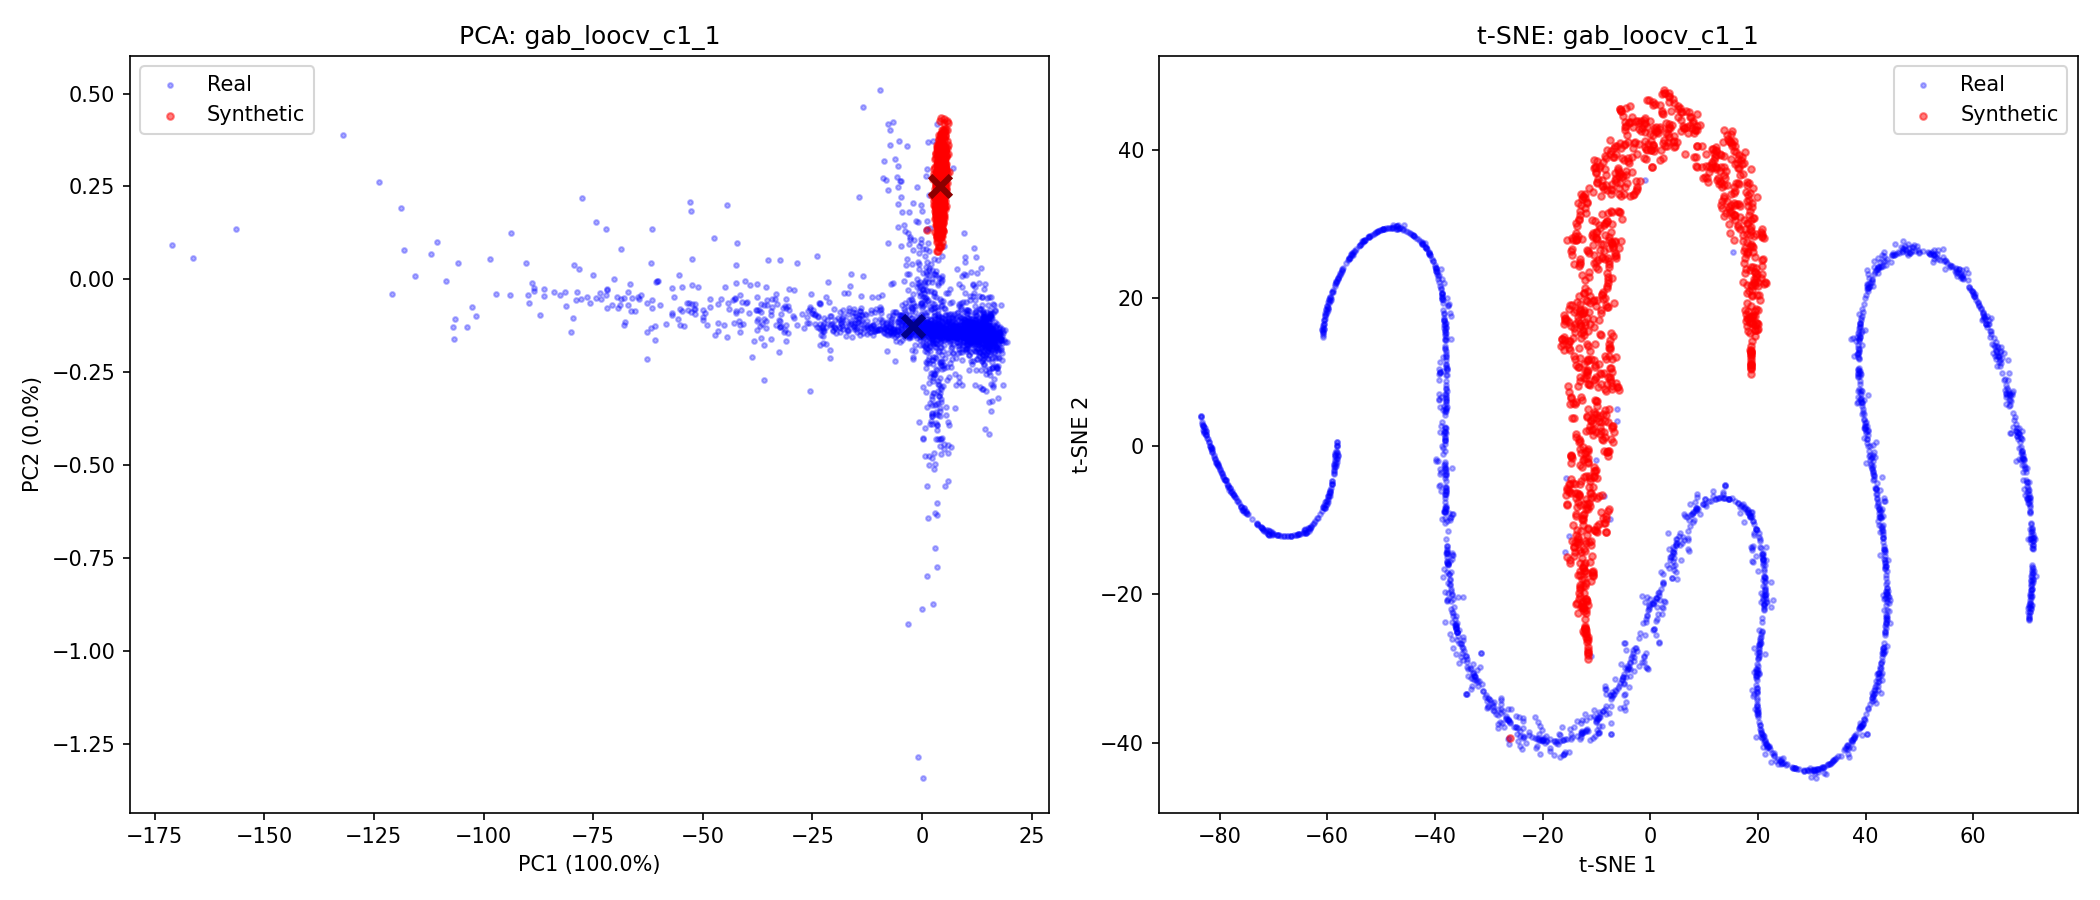
\includegraphics[width=\textwidth]{figures/gab_loocv_c1_1_gcn_visualization.png}
		\caption{Config 1, NM=1 (LR=0.001)}
	\end{subfigure}
	\hfill
	\begin{subfigure}[b]{0.48\textwidth}
		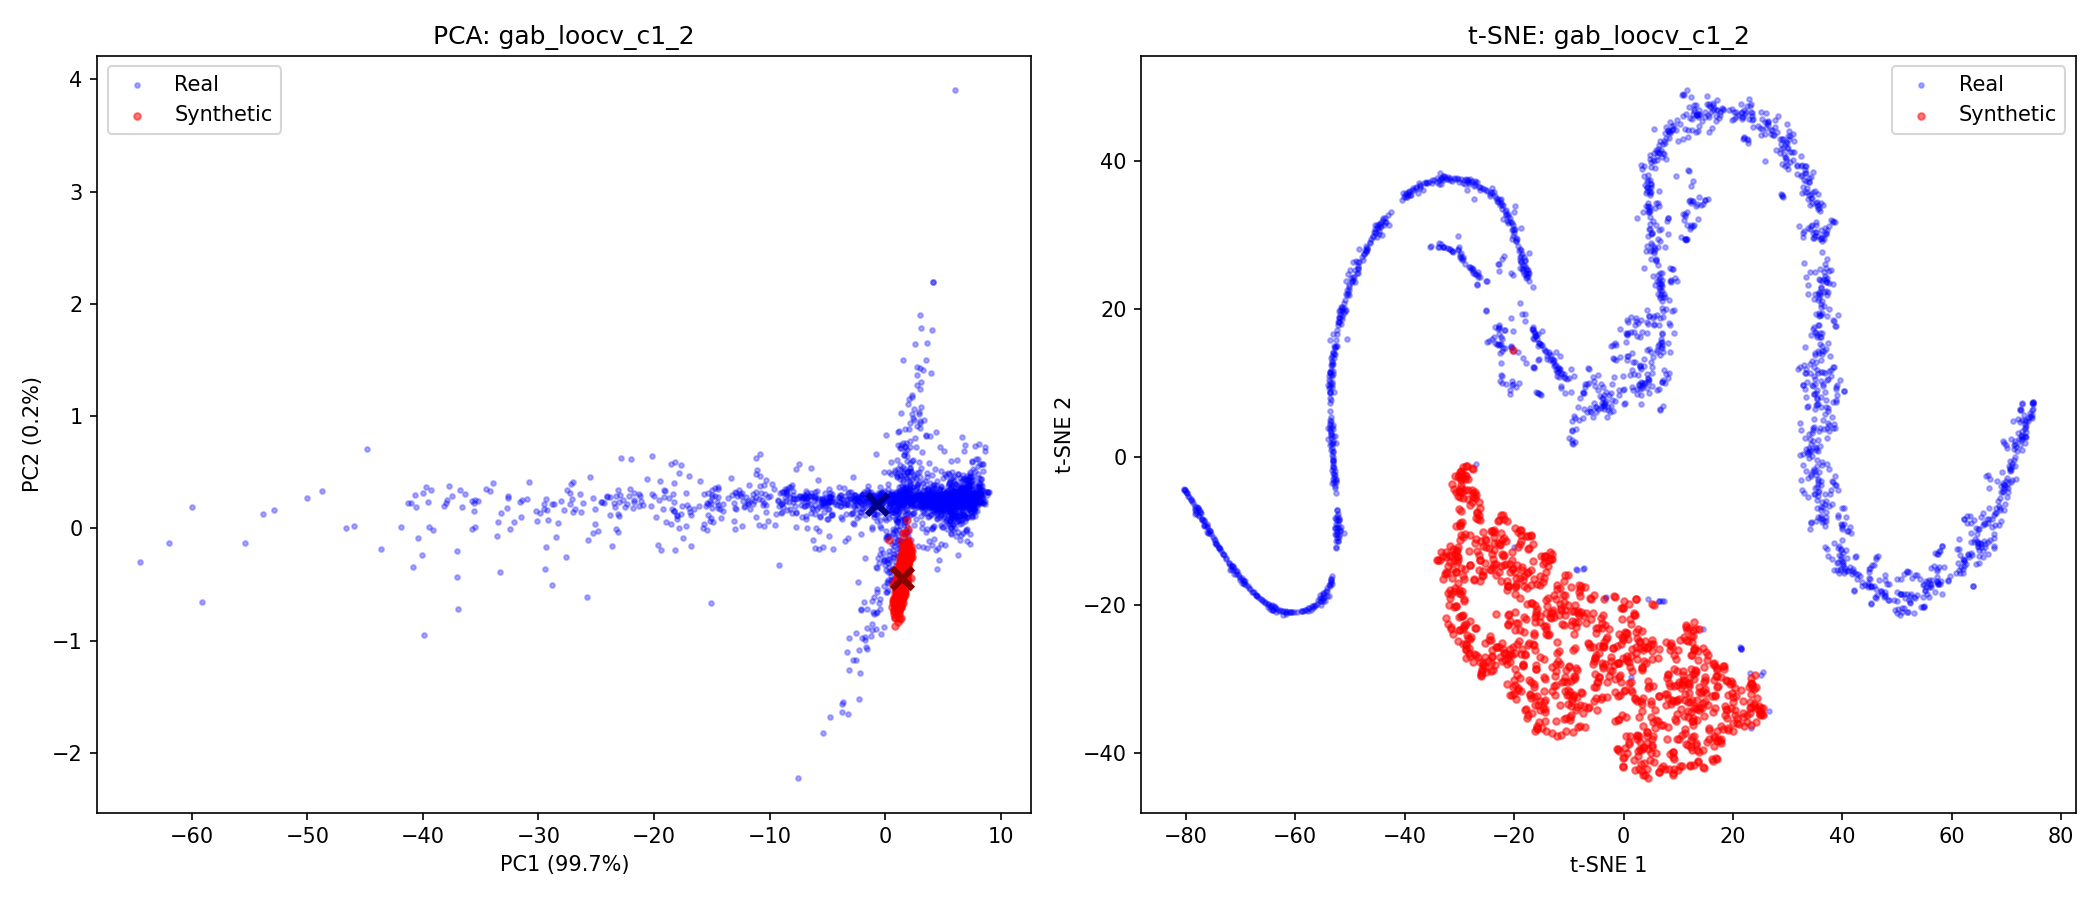
\includegraphics[width=\textwidth]{figures/gab_loocv_c1_2_gcn_visualization.png}
		\caption{Config 1, NM=2 (LR=0.001)}
	\end{subfigure}

	\vspace{0.5em}

	\begin{subfigure}[b]{0.48\textwidth}
		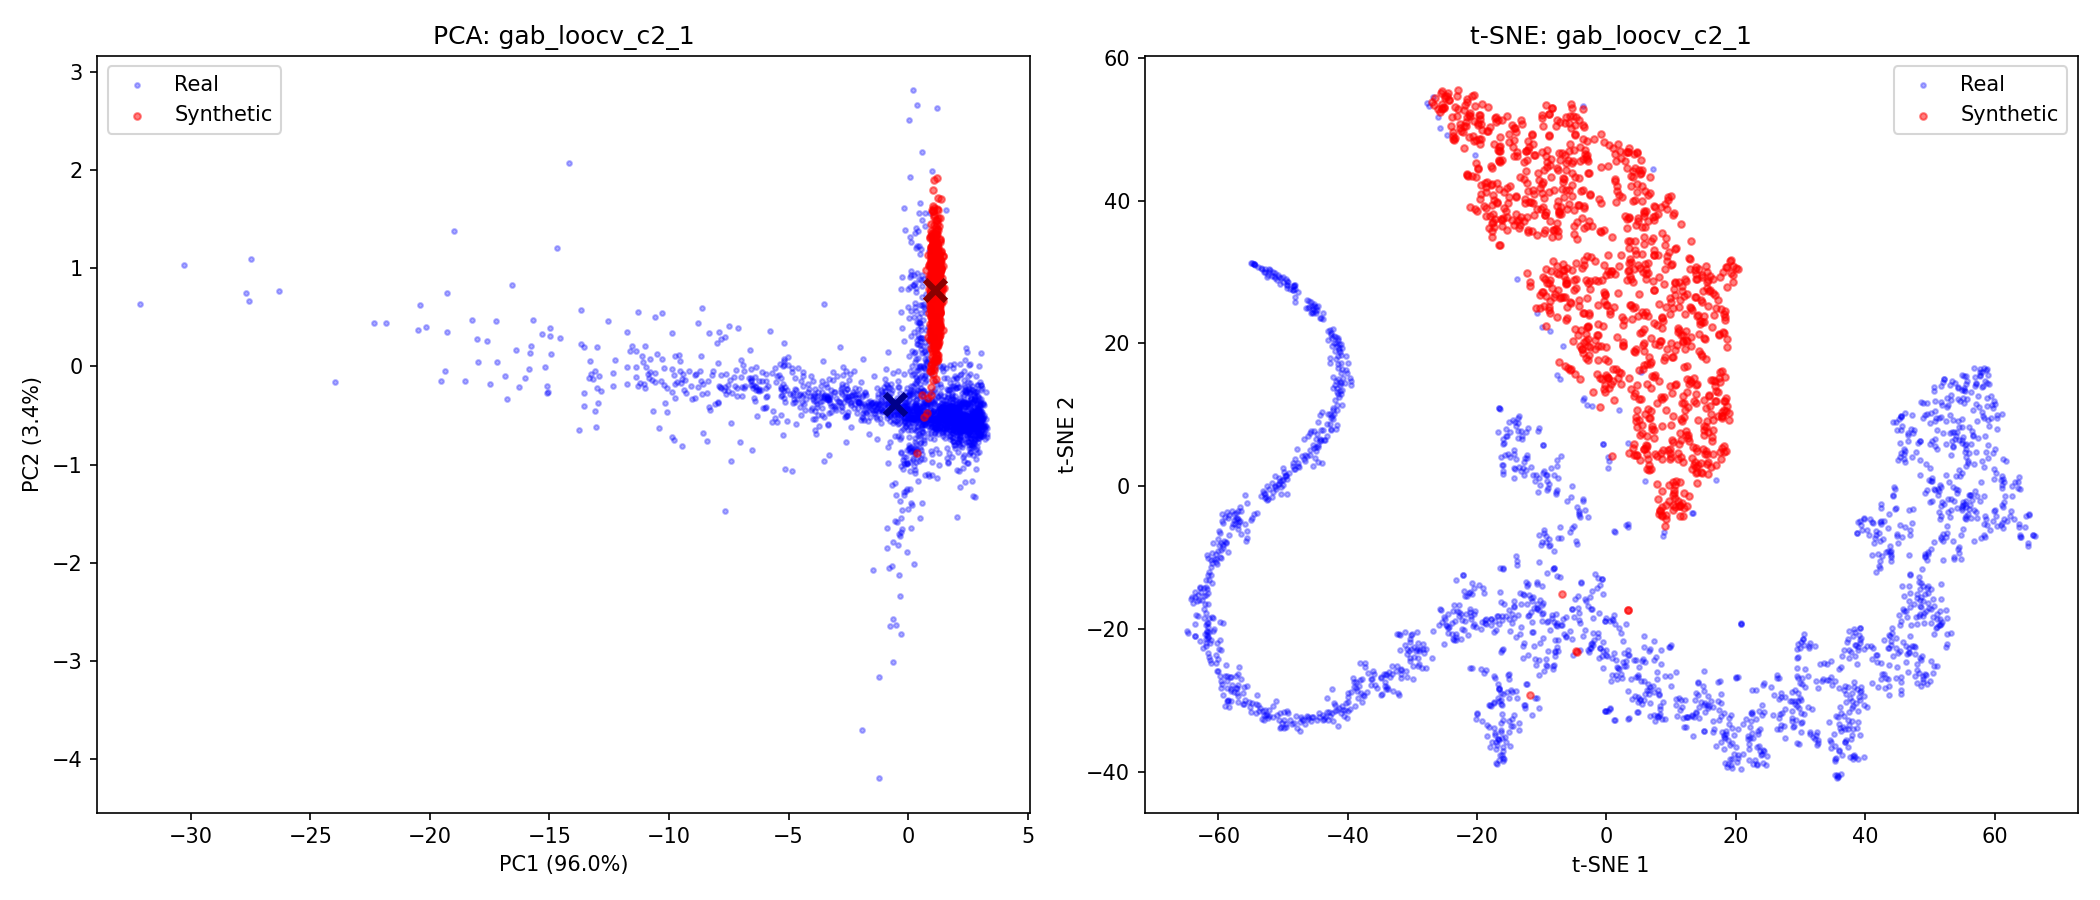
\includegraphics[width=\textwidth]{figures/gab_loocv_c2_1_gcn_visualization.png}
		\caption{Config 2, NM=1 (LR=0.0005)}
	\end{subfigure}
	\hfill
	\begin{subfigure}[b]{0.48\textwidth}
		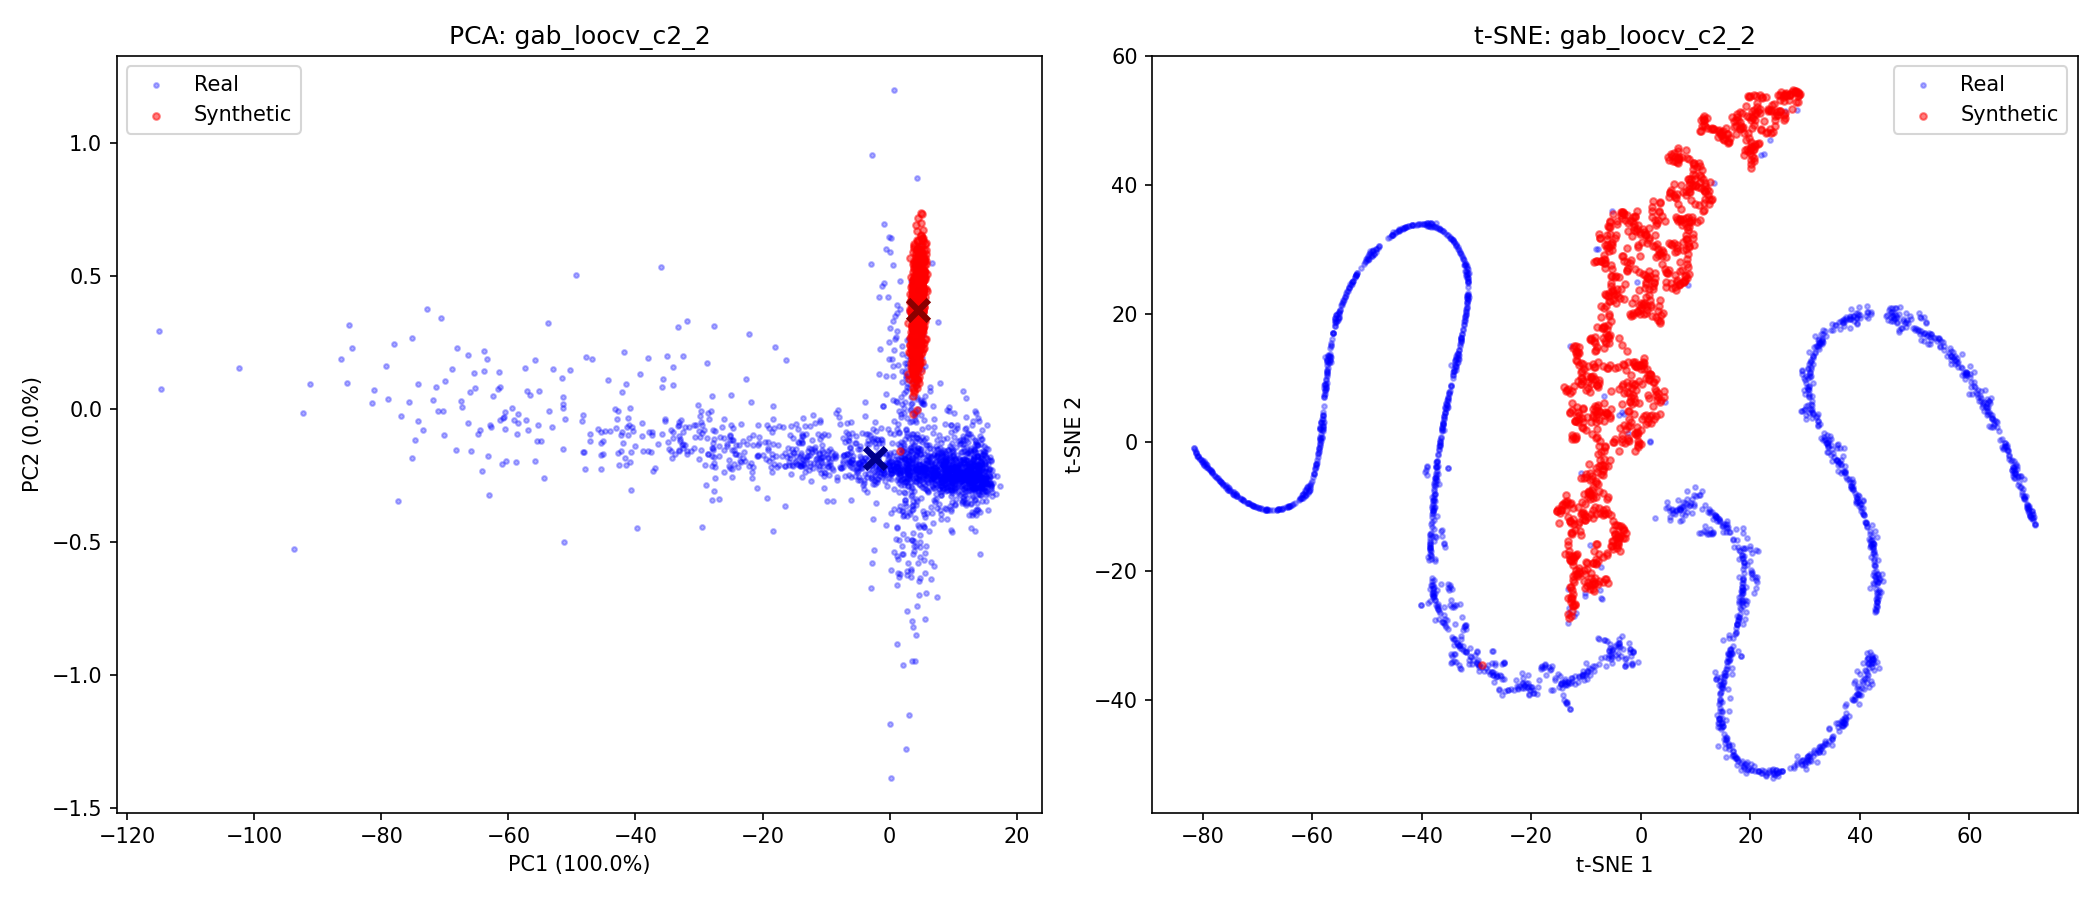
\includegraphics[width=\textwidth]{figures/gab_loocv_c2_2_gcn_visualization.png}
		\caption{Config 2, NM=2 (LR=0.0005)}
	\end{subfigure}
	\caption{PCA and t-SNE visualization of GCN embeddings for Original implementation. Blue points represent real users, red points represent synthetic users.}
	\label{fig:gcn_original}
\end{figure}

\begin{figure}[H]
	\centering
	\begin{subfigure}[b]{0.48\textwidth}
		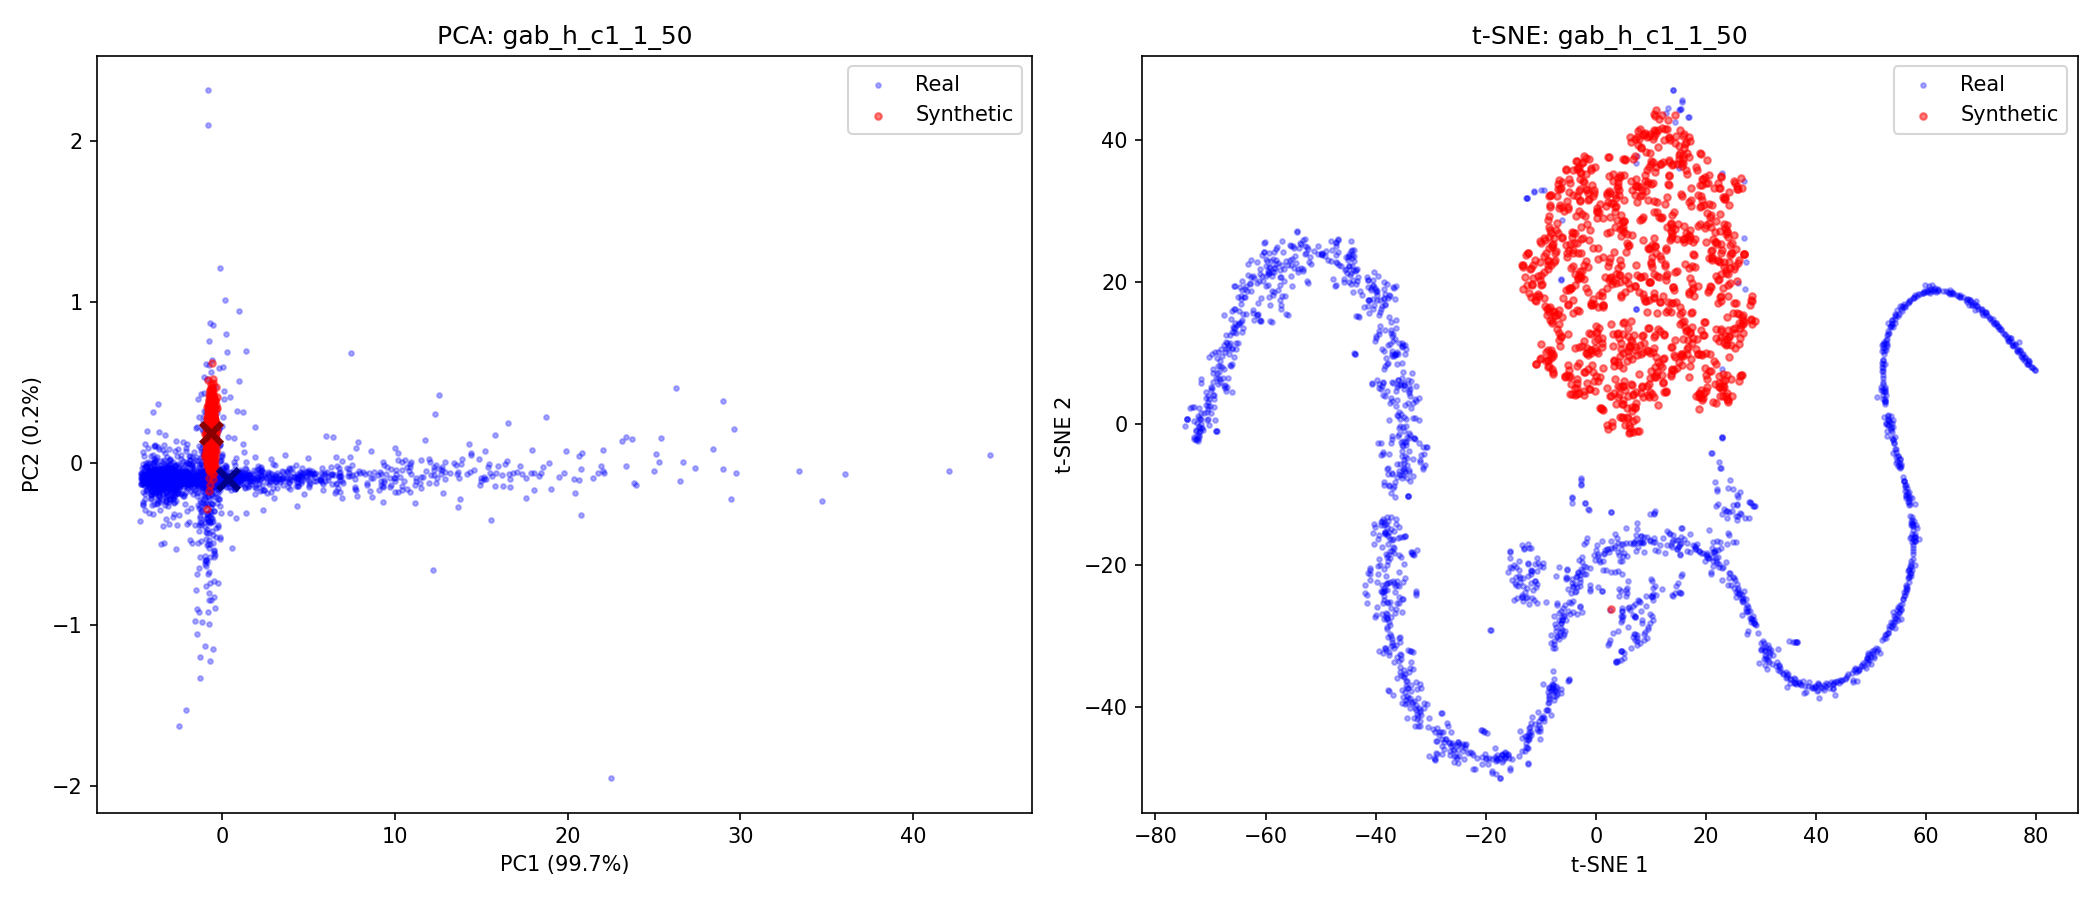
\includegraphics[width=\textwidth]{figures/gab_h_c1_1_50_gcn_visualization.png}
		\caption{Config 1, NM=1 (LR=0.001)}
	\end{subfigure}
	\hfill
	\begin{subfigure}[b]{0.48\textwidth}
		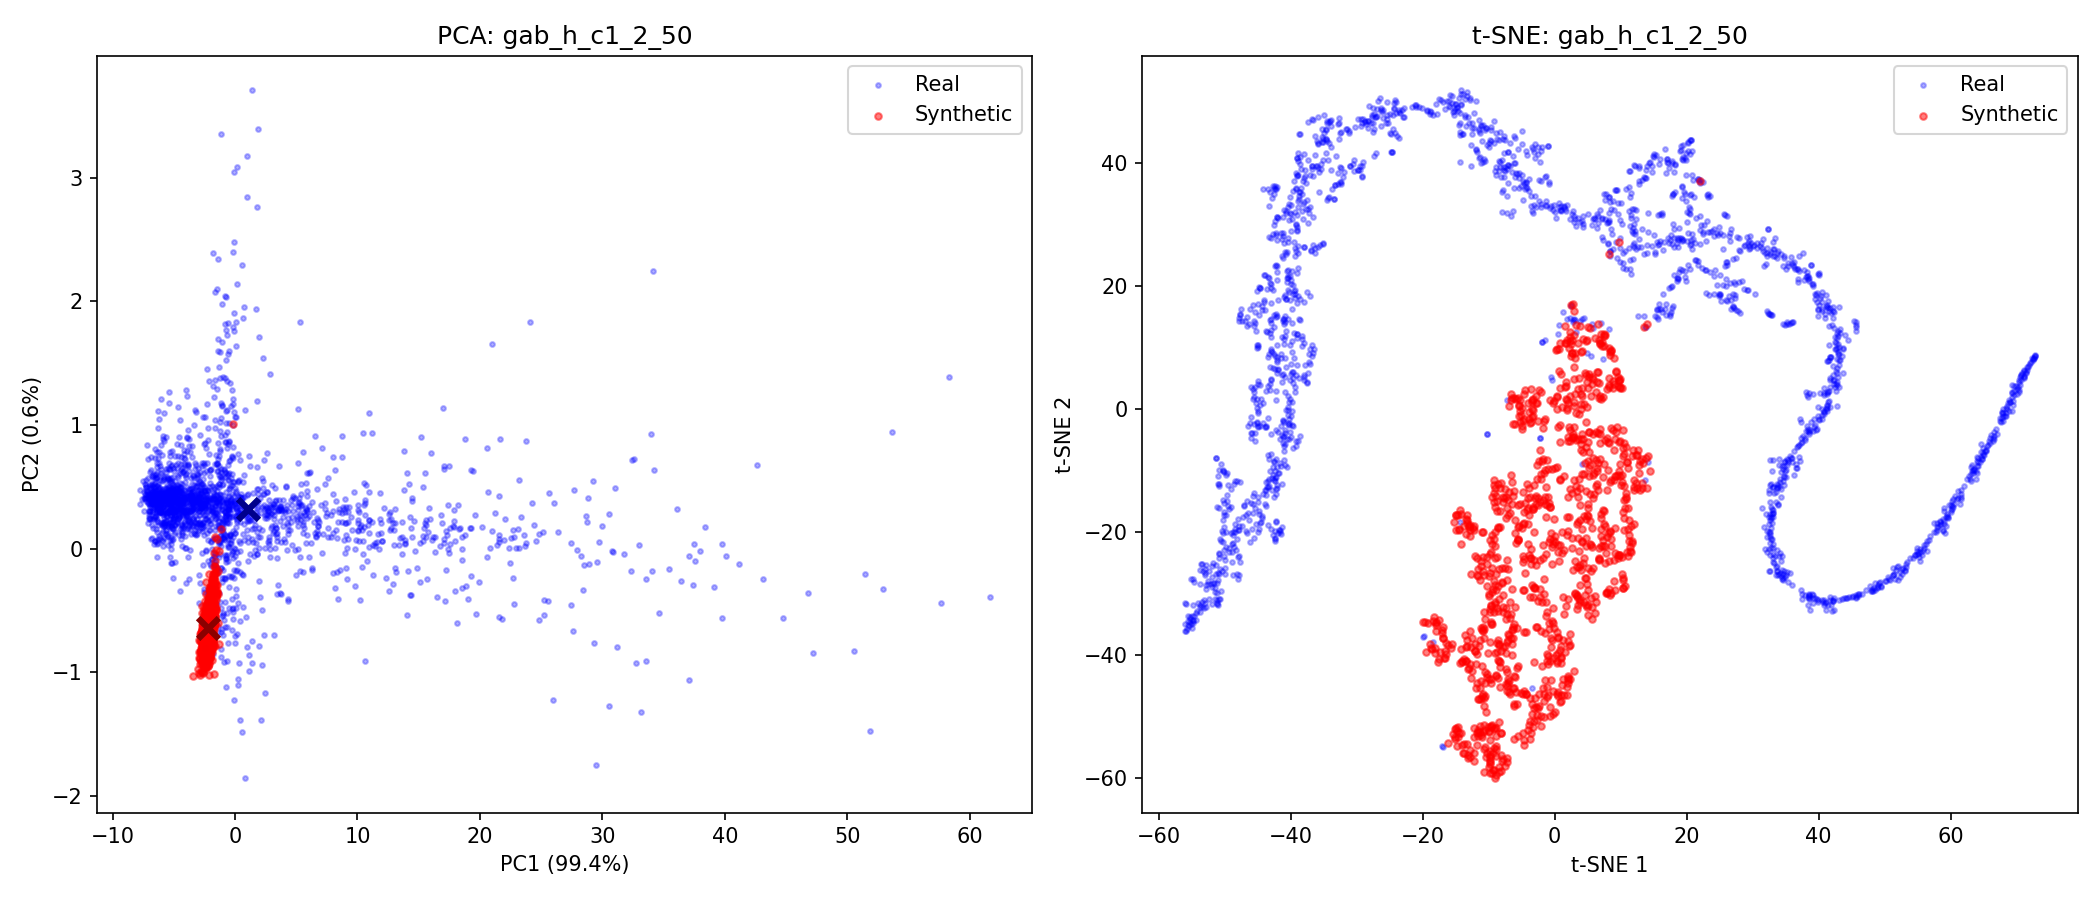
\includegraphics[width=\textwidth]{figures/gab_h_c1_2_50_gcn_visualization.png}
		\caption{Config 1, NM=2 (LR=0.001)}
	\end{subfigure}

	\vspace{0.5em}

	\begin{subfigure}[b]{0.48\textwidth}
		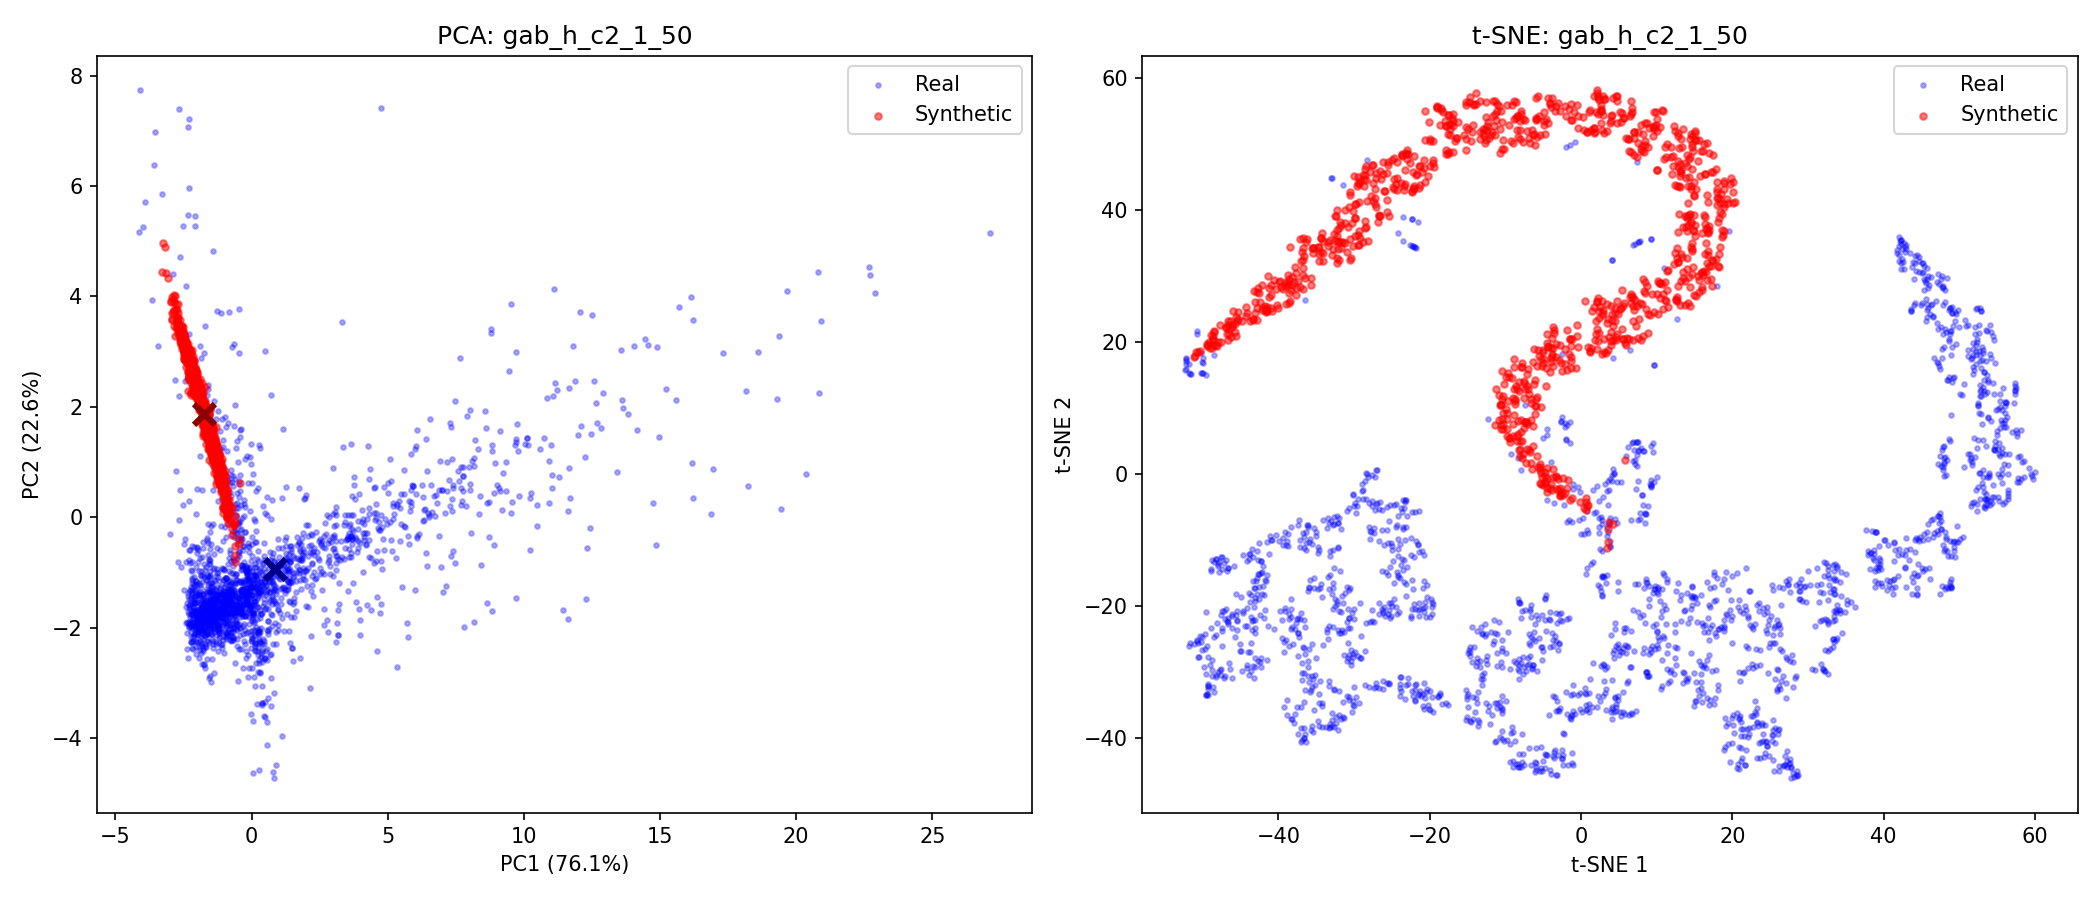
\includegraphics[width=\textwidth]{figures/gab_h_c2_1_50_gcn_visualization.png}
		\caption{Config 2, NM=1 (LR=0.0005)}
	\end{subfigure}
	\hfill
	\begin{subfigure}[b]{0.48\textwidth}
		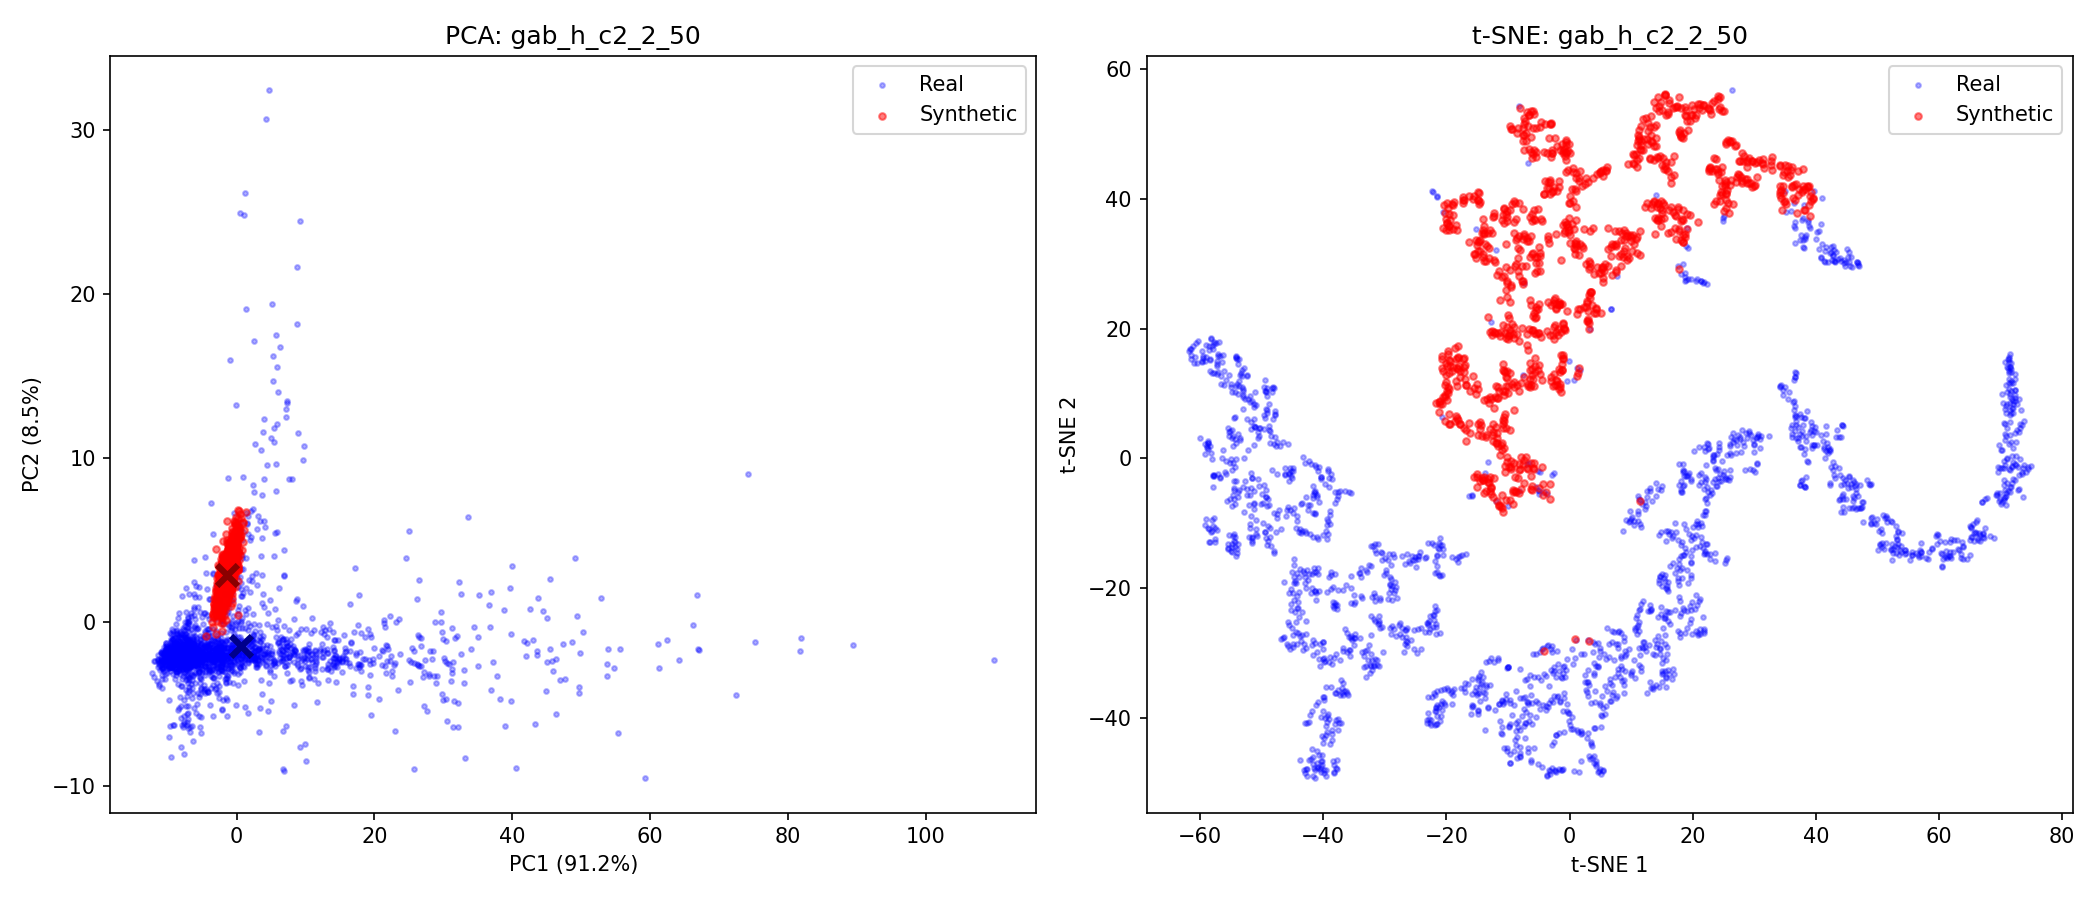
\includegraphics[width=\textwidth]{figures/gab_h_c2_2_50_gcn_visualization.png}
		\caption{Config 2, NM=2 (LR=0.0005)}
	\end{subfigure}
	\caption{PCA and t-SNE visualization of GCN embeddings for Incremental implementation. Blue points represent real users, red points represent synthetic users.}
	\label{fig:gcn_incremental}
\end{figure}

Table~\ref{tab:pca_stats} summarizes the PCA statistics for each configuration, including the explained variance ratio and the centroid distance between real and synthetic user embeddings.

\begin{table}[h]
	\centering
	\caption{PCA statistics for GCN embeddings}
	\label{tab:pca_stats}
	\small
	\begin{tabular}{llcccc}
		\toprule
		 & \textbf{Config} & \textbf{PC1}       & \textbf{PC2}       & \textbf{Total}     & \textbf{Centroid} \\
		 &                 & \textbf{Explained} & \textbf{Explained} & \textbf{Explained} & \textbf{Distance} \\
		\midrule
		\multirow{4}{*}{\rotatebox{90}{\textbf{Orig.}}}
		 & Config 1, NM=1  & 99.98\%            & 0.01\%             & 100.00\%           & 6.29              \\
		 & Config 1, NM=2  & 99.71\%            & 0.23\%             & 99.94\%            & 2.33              \\
		 & Config 2, NM=1  & 95.99\%            & 3.39\%             & 99.38\%            & 2.06              \\
		 & Config 2, NM=2  & 99.96\%            & 0.03\%             & 100.00\%           & 6.65              \\
		\midrule
		\multirow{4}{*}{\rotatebox{90}{\textbf{Incr.}}}
		 & Config 1, NM=1  & 99.65\%            & 0.21\%             & 99.86\%            & 1.01              \\
		 & Config 1, NM=2  & 99.39\%            & 0.57\%             & 99.96\%            & 3.41              \\
		 & Config 2, NM=1  & 76.13\%            & 22.61\%            & 98.74\%            & 3.84              \\
		 & Config 2, NM=2  & 91.20\%            & 8.47\%             & 99.67\%            & 4.78              \\
		\bottomrule
	\end{tabular}
\end{table}

The analysis reveals several key observations:

\paragraph{Dimensional Collapse and Oversmoothing.} The Original implementation configurations show extreme concentration in the first principal component (95-100\%), indicating \textbf{dimensional collapse}: the GCN embeddings collapse to a nearly one-dimensional space. This phenomenon is closely related to \textbf{oversmoothing} in Graph Neural Networks, where repeated message passing operations cause node representations to become indistinguishable from one another \cite{liDeeperInsightGraph2018,oonoGraphNeuralNetworks2020}. After multiple GCN layers, each node's embedding becomes dominated by the aggregated neighborhood statistics rather than its individual features.

In contrast, the Incremental implementation shows more variance distribution: Config 2 with NM=1 achieves only 76.13\% on PC1, with 22.61\% on PC2, suggesting a richer embedding space with less severe oversmoothing. This may explain why that particular run is the only one that attempts to connect synthetic users, even if with poor performance.

\paragraph{Centroid Distance.} The centroid distance between real and synthetic embeddings correlates strongly with classification performance:
\begin{itemize}
	\item \textbf{Original Config 1 NM=1 (6.29)} and \textbf{Config 2 NM=2 (6.65)}: Excellent separation, aligning with the highest MAP scores (0.8660) and balanced F1.
	\item \textbf{Incremental Config 1 NM=1 (1.01)}: Poor separation, correlated to the fact that the model predicts exclusively Class 1.
	\item \textbf{Incremental Config 2 NM=1 (3.84)} and \textbf{Config 2 NM=2 (4.78)}: Moderate separation with richer embedding structure (lower PC1 explained variance).
\end{itemize}

We can say that the failure in connecting synthetic users for the original configurations is due to the fact that the model learns a very narrow embedding space where real and synthetic users are perfectly separated, but the synthetic users are clustered in a single point, so the model is not able to learn any discriminative feature for them, and it ends up predicting always 0 for the edges between synthetic users. On the other hand, the incremental approach that link synthetic users is the one with the lowest explained variance on PC1, and the highest explained variance on PC2, so the model learns a richer embedding space where real and synthetic users are not perfectly separated, but the synthetic users are spread across the space, so the model is able to learn some discriminative features for them, even if with poor performance.

\paragraph{Effect of Negative Sampling.} Increasing NM from 1 to 2 generally improves centroid distance separation, particularly for the Incremental approach (1.01 $\rightarrow$ 3.41 for Config 1). This confirms that higher negative sampling encourages the model to learn more discriminative features.

% \paragraph{Original vs. Incremental Trade-off.} The Original approach achieves better separation (higher centroid distances) but with collapsed embedding dimensions. The Incremental approach produces more distributed embeddings but struggles with class separation, particularly with low negative sampling. This suggests a trade-off between embedding richness and discriminative power.

% The t-SNE visualizations complement these findings: real users form dense central clusters in configurations with high explained variance on PC1, while synthetic users spread across the periphery.

% \subsection*{Link Prediction Task}

% \subsection*{Populating the synthetic graph}

% \subsection*{Network metrics}

% Table~\ref{tab:social_network_metrics} presents the graph structural metrics for the Gab dataset compared to established social network datasets (Facebook, Twitter, Google+). The metrics include the number of nodes and edges, average degree, average path length, modularity, and clustering coefficient.

% \begin{table}[H]
% 	\centering
% 	\caption{Structural metrics comparison}
% 	\label{tab:social_network_metrics}
% 	\begin{tabular}{
% 			l
% 			S[table-format=5.0]
% 			S[table-format=8.0]
% 			S[table-format=2.2]
% 			S[table-format=1.2]
% 			S[table-format=1.2]
% 			S[table-format=1.2]
% 		}
% 		\toprule
% 		\textbf{Network}        &
% 		\textbf{Nodes}          &
% 		\textbf{Edges}          &
% 		\textbf{Avg Deg}        &
% 		\textbf{Avg Path}       &
% 		\textbf{Mod}            &
% 		\textbf{Clust. Coef.}                                                     \\
% 		\midrule
% 		Facebook                & 4039   & 88234    & 43.69  & 3.69 & 0.83 & 0.61 \\
% 		Twitter                 & 81306  & 1768149  & 21.75  & 4.91 & 0.80 & 0.57 \\
% 		Google+\footnotemark[4] & 107614 & 13673453 & 127.06 & 3.32 & 0.47 & 0.49 \\
% 		Gab (Ours)              & 25569  & 820910   & 32.11  & 3.08 & 0.24 & 0.08 \\
% 		\bottomrule
% 	\end{tabular}
% \end{table}
% \footnotetext[1]{https://snap.stanford.edu/data/ego-Facebook.html}
% \footnotetext[2]{https://snap.stanford.edu/data/ego-Twitter.html}
% \footnotetext[3]{https://snap.stanford.edu/data/ego-Gplus.html}
% \footnotetext[4]{Due to the dimension of the Google+ dataset, we report the metrics for the largest connected component (LCC) considering the 20\% of nodes with the highest degree.}

% The Gab dataset exhibits notably lower clustering coefficient (0.08) compared to other social networks (0.49-0.61), suggesting weaker local community structure and less triadic closure. The modularity of 0.24 is also lower than Facebook (0.83) and Twitter (0.80), indicating weaker community boundaries. However, the average path length of 3.08 is comparable to Facebook (3.69) and Google+ (3.32), confirming the ``small-world'' property typical of social networks.

% The lower clustering and modularity may reflect:
% \begin{itemize}
% 	\item The platform's specific user demographics and community structure
% 	\item Different interaction patterns compared to mainstream social networks
% 	\item The minimal content moderation creating different connection dynamics
% \end{itemize}

% Results from the experiments will be reported in this section once the training is completed. The evaluation will compare:
% \begin{itemize}
% 	\item The cumulative (standard) approach vs. the incremental approach
% 	\item Different feature configurations (degree-based vs. embedding-based)
% 	\item Both EvolveGCN-H and EvolveGCN-O variants where feasible
% \end{itemize}

% The structural properties of generated synthetic networks will be compared against the original Gab dataset and the baseline social networks shown in Table~\ref{tab:baseline_metrics}.


% \section{Evaluate Results}

% The evaluation assesses the extent to which the project meets the business success criteria defined in Chapter~\ref{cha:businessunderstanding}.

% \subsection*{Business Success Criteria Assessment}

% The business success criteria from Section~\ref{sec:business_success} are evaluated as follows:

% \begin{itemize}
% 	\item \textbf{Development of a temporal link prediction model based on EvolveGCN}: The model architecture has been implemented following the EvolveGCN-H variant, with support for both standard and incremental training pipelines.

% 	\item \textbf{Quantitative comparison using standard metrics}: The evaluation framework computes AUC-ROC, MAP, Precision, Recall, and F1-score as specified. Results are reported in Table~\ref{tab:results_comparison}, with the best configuration achieving MAP of 0.8660 (Original) and AUC of 0.8037 (Incremental).

% 	\item \textbf{Transfer learning for synthetic network generation}: The model can generate edge predictions on synthetic datasets, with structural analysis comparing degree distribution, clustering coefficient, average path length, and modularity against real networks. \textit{Status: Implementation complete, evaluation pending.}

% 	\item \textbf{Analysis of network evolution patterns}: The incremental training pipeline captures temporal dynamics through phase-by-phase adaptation. \textit{Status: Achieved.}

% 	\item \textbf{Generation of 1000-user synthetic network}: This objective requires completing experiments on the synthetic datasets. \textit{Status: Pending.}
% \end{itemize}

% \subsection*{Data Mining Success Criteria Assessment}

% The data mining success criteria from Section~\ref{sec:datamining_success} are evaluated:

% \begin{itemize}
% 	\item \textbf{High performance on link prediction tasks}: The best Original configuration achieves MAP of 0.8660 and Macro F1 of 0.8631, while the best Incremental configuration achieves AUC of 0.8037. Both approaches demonstrate effective temporal link prediction, with the Original approach showing superior classification performance and the Incremental approach showing better ranking quality (AUC).

% 	\item \textbf{Generalization to synthetic datasets}: The structural metrics comparison framework is in place. Generated networks will be evaluated for realism against Facebook, Twitter, Google+, and the original Gab network baselines.

% 	\item \textbf{Comprehensive insights on structural properties}: The GraphMetricsCalculator module computes all required metrics (average degree, clustering coefficient, modularity, shortest path length, community count).
% \end{itemize}



% \section{Review Process}

% The evaluation process follows an iterative approach:

% \begin{enumerate}
% 	\item \textbf{Phase-by-phase Review}: Each incremental training phase is reviewed immediately after completion, allowing for hyperparameter adjustments before the next phase.

% 	\item \textbf{Cross-validation}: For the standard approach, k-fold cross-validation ensures robustness of reported metrics.

% 	\item \textbf{Baseline Comparison}: Performance is compared against simple baselines:
% 	      \begin{itemize}
% 		      \item Random edge prediction
% 		      \item Preferential attachment (popular nodes get more connections)
% 		      \item Common neighbors heuristic (triadic closure)
% 	      \end{itemize}

% 	\item \textbf{Statistical Significance}: Bootstrap confidence intervals are computed for all metrics to assess reliability.
% \end{enumerate}



% \section{Determine Next Steps}

% Based on the current project status, the following next steps are recommended:

% \begin{enumerate}
% 	\item Complete training experiments on all six temporal snapshots
% 	\item Generate and evaluate synthetic networks using the trained models
% 	\item Compare incremental vs. standard approaches across all evaluation dimensions
% 	\item Document final results and prepare for potential deployment considerations
% \end{enumerate}